\documentclass[graphics]{beamer}

\usepackage{graphicx}
\usepackage{verbatim}
\usepackage{wrapfig}
\useoutertheme{shadow}
%\usecolortheme{orchid}
\usecolortheme{seahorse}


% math commands
\newcommand{\be}{\begin{eqnarray}}
\newcommand{\ee}{\end{eqnarray}}
\newcommand{\beq}{\begin{equation}}
\newcommand{\eeq}{\end{equation}}
\def\simless{\mathbin{\lower 3pt\hbox
      {$\rlap{\raise 5pt\hbox{$\char'074$}}\mathchar"7218$}}}
\def\simgreat{\mathbin{\lower 3pt\hbox
      {$\rlap{\raise 5pt\hbox{$\char'076$}}\mathchar"7218$}}} %> or of order

% variables

\def\toonscale{0.45}
\def\mboxy#1{\mbox{\small #1}}


\begin{comment}
\AtBeginSection[]{
  \frame{
    \frametitle{Outline}
    \tableofcontents[currentsection]
  }
}
\end{comment}

\title{21cm intensity mapping: current results and future potential
}
\subtitle{interim update}
\author[U. Pen]{Ue-Li Pen, Toronto
\\[8mm] 
}
\date{June 29, 2016}


\begin{document}

%\section*{Introduction}
\section{Current results}

\begin{comment}
  \subsection{Outline}

  \frame{
    \frametitle{Outline}
    \tableofcontents
  }
\end{comment}

\frame{\maketitle}



  \frame{
\vspace{-0.5in}
    \frametitle{History}
    \begin{itemize}
        \item Intensity mapping: LSS using HI in galaxies without
          detecting individual galaxies
        \item morales-Whythe
        \item Chang et al 2008
        \item mushrooming of dedicated experiments
%          \vspace{-0.15in}
    \end{itemize}
\vspace{-0.1in}\hspace{.3in}
\includegraphics[width=1.2in]{Figures/gbt.jpg}
\vspace{-0.5in}
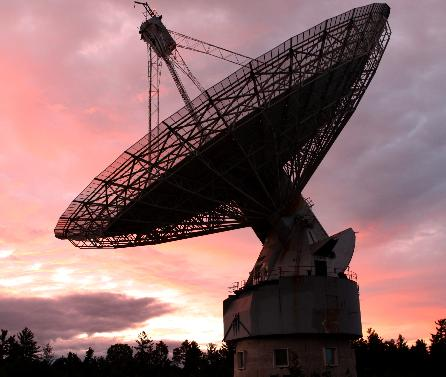
\includegraphics[width=1.9in]{Figures/IMG-7749-ARO-crop.JPG}
  }


  \frame{
\vspace{-0.5in}
    \frametitle{GBT-IM}
    \begin{itemize}
        \item 650 hours in 700-900 MHz band
        \item initial power spectrum: cross correlation with WiggleZ,
          auto spectrum
        \item measures $\Omega_{HI}b$ (Masui et al, Switzer et al)
        \item archival discovery of FRB110523
%          \vspace{-0.15in}
    \end{itemize}
\vspace{-0.1in}\hspace{.3in}
\includegraphics[width=1.2in]{Figures/gbt.jpg}
\vspace{-0.5in}
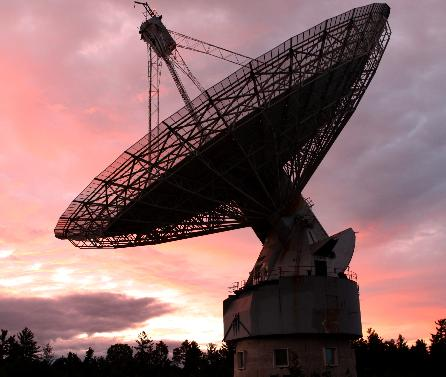
\includegraphics[width=1.9in]{Figures/IMG-7749-ARO-crop.JPG}
  }

  \frame{
\vspace{-0.5in}
    \frametitle{Parkes-IM}
    \begin{itemize}
      \item 500 beam-hours on 2dF field
      \item measure 21cm auto-power, cross-power, RSD, $\Omega_{HI}$
      \item analysis in progress
%          \vspace{-0.15in}
    \end{itemize}
\vspace{-0.1in}\hspace{.3in}
\includegraphics[width=1.9in]{Figures/Parkes.png}
\vspace{-0.5in}
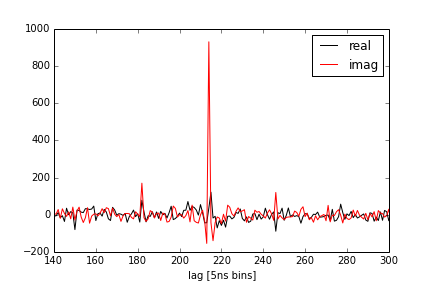
\includegraphics[width=1.9in]{Figures/ARO-DRAO-lf-zoom.png}
  }

\section{Experiments under construction}
  \frame{
    \frametitle{CHIME}
    \begin{itemize}
        \item Pathfinder operating: sky maps
        \item Full CHIME construction completed, 
    \end{itemize}
\vspace{-0.1in}\hspace{.3in}
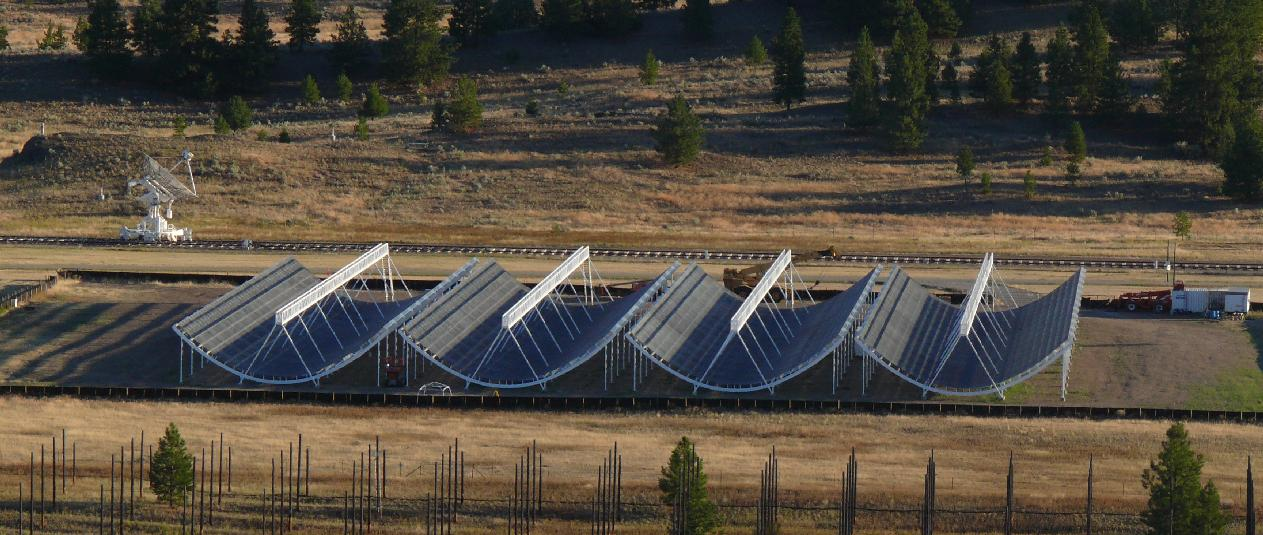
\includegraphics[width=1.9in]{Figures/Chime-medium.jpg}
}
  \frame{
    \frametitle{Tianlai}
    \begin{itemize}
        \item in Xinjian, China
        \item 
    \end{itemize}
\vspace{-0.1in}\hspace{.3in}
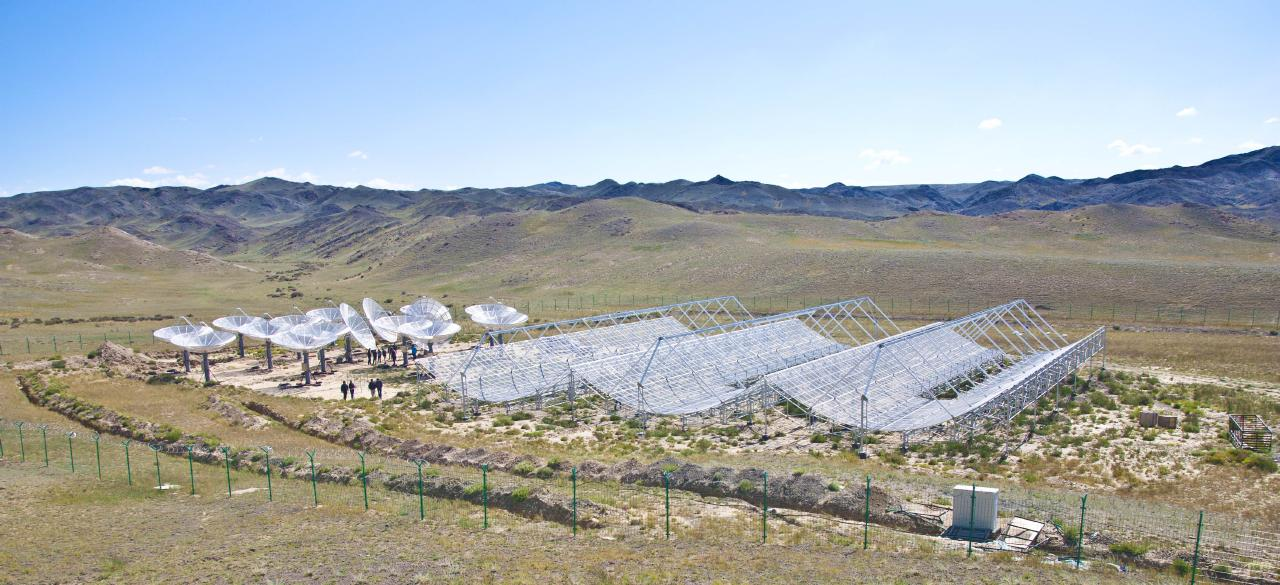
\includegraphics[width=1.9in]{Figures/tianlai-medium.jpg}
}

  \frame{
    \frametitle{HIRAX}
    \begin{itemize}
        \item Karoo, SA
        \item most ambitious IM-BAO project, doubles as pulsar and FRB engine
    \end{itemize}
\vspace{-0.1in}\hspace{.3in}
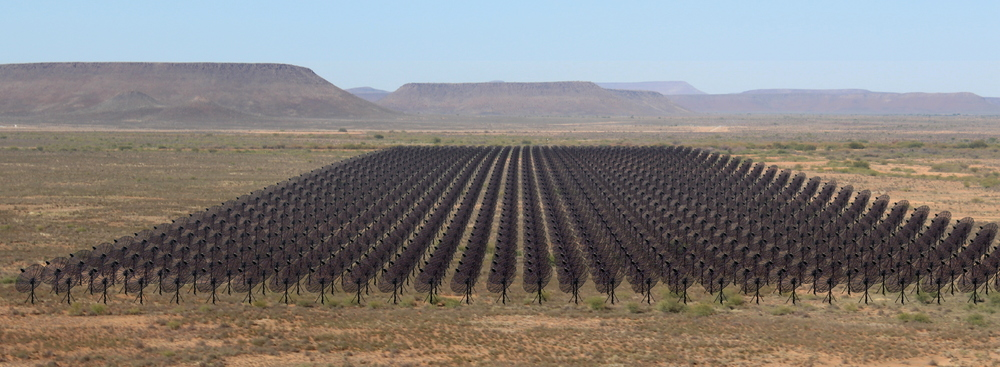
\includegraphics[width=1.9in]{Figures/hirax-karoo-s.jpg}
}
\section{Future Experiments}
  \frame{
    \frametitle{Proposed/Planned}
    \begin{itemize}
        \item BINGO, BAOBAB
        \item CO, L$_\alpha$, other lines
    \end{itemize}
  \frame{
    \frametitle{Outlook}
    \begin{itemize}
        \item 21cm signal-foreground sweetspots: $z<2,\ z \sim 8, z
          \sim 15$
        \item figure from pritchard et al
        \item FAST aperture array, cylinder array
    \end{itemize}

}

\end{document}
